\section{Wm4Math\-MCR.h File Reference}
\label{Wm4MathMCR_8h}\index{Wm4MathMCR.h@{Wm4MathMCR.h}}


This graph shows which files directly or indirectly include this file:\begin{figure}[H]
\begin{center}
\leavevmode
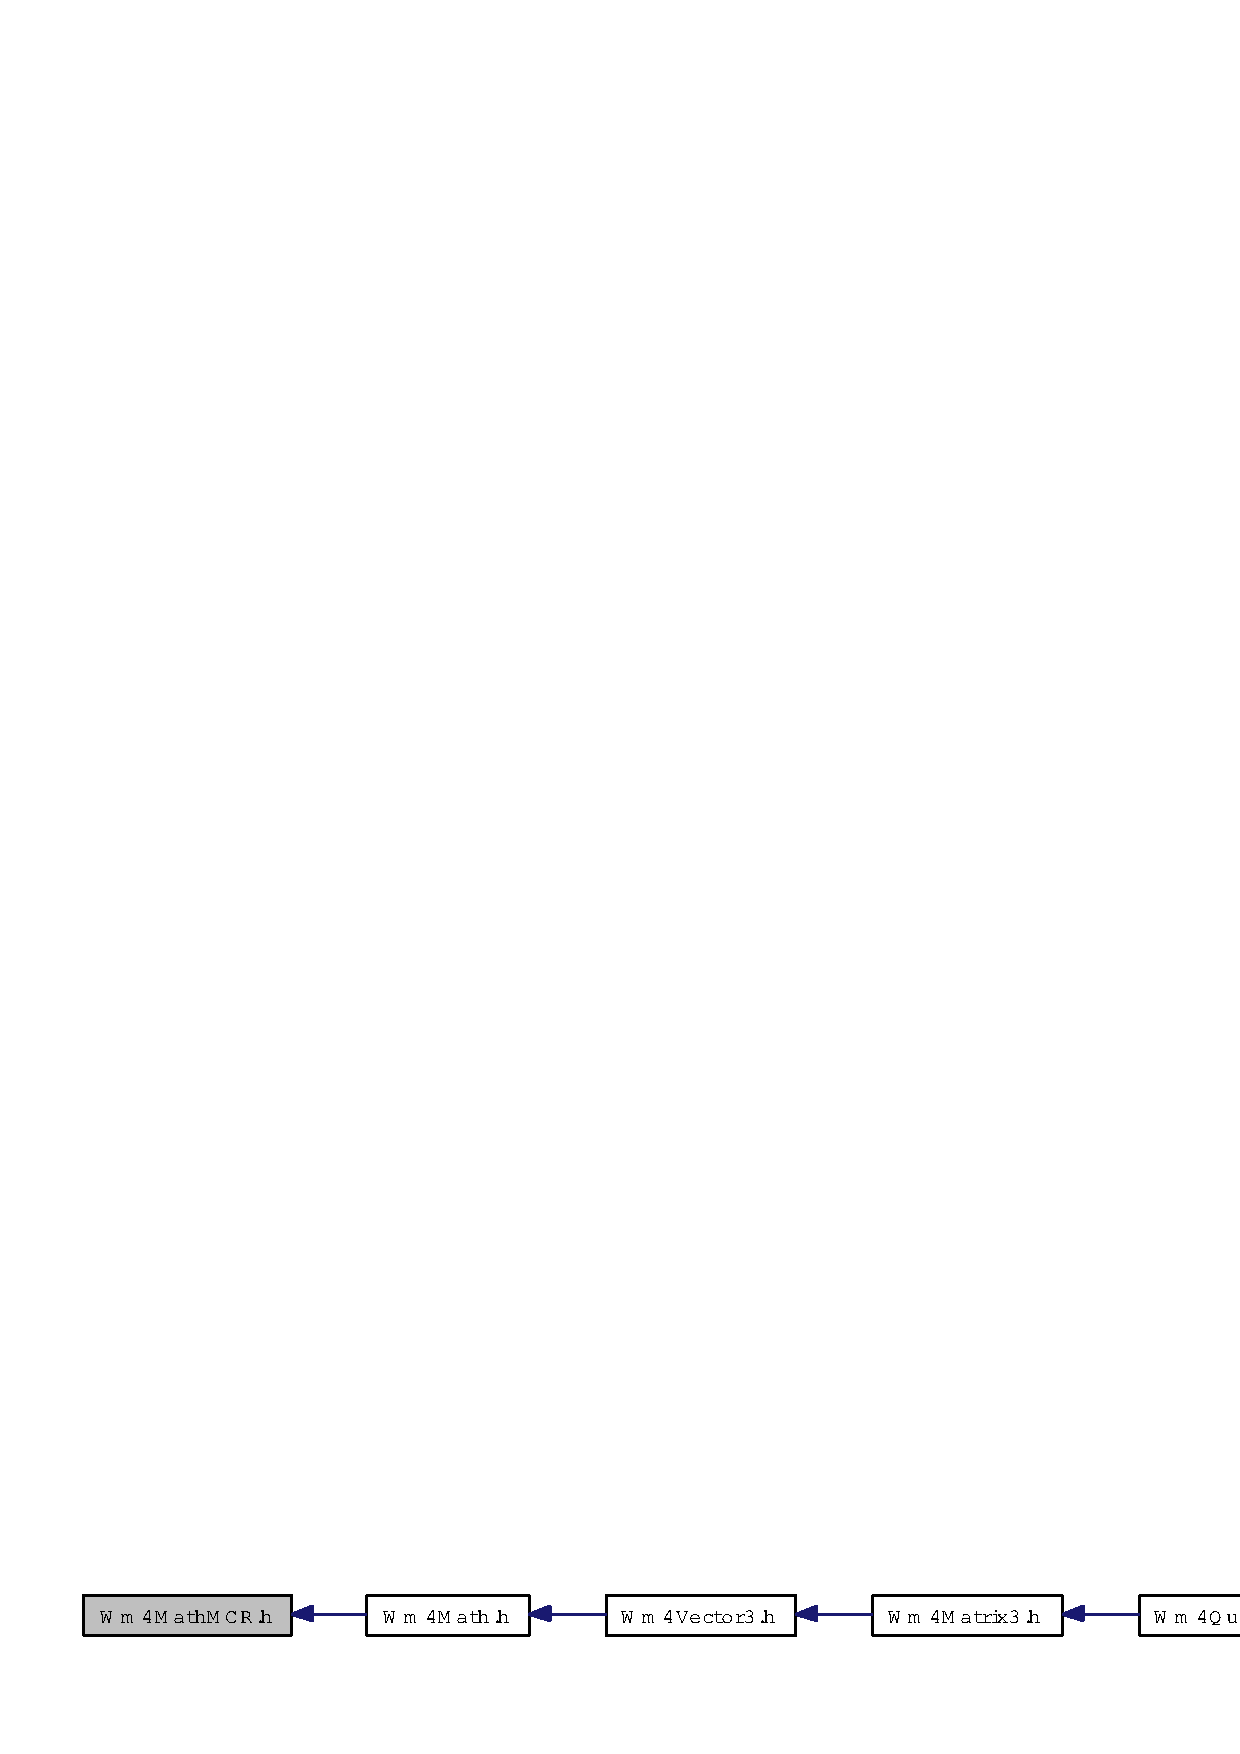
\includegraphics[width=405pt]{Wm4MathMCR_8h__dep__incl}
\end{center}
\end{figure}
\subsection*{Defines}
\begin{CompactItemize}
\item 
\#define {\bf WM4\_\-SCALED\_\-FLOAT\_\-TO\_\-INT}(f\-Float, i\-Log, i\-Int)
\item 
\#define {\bf WM4\_\-SCALED\_\-FLOAT\_\-TO\_\-INT}(f\-Float, i\-Log, i\-Int)
\end{CompactItemize}


\subsection{Define Documentation}
\index{Wm4MathMCR.h@{Wm4Math\-MCR.h}!WM4_SCALED_FLOAT_TO_INT@{WM4\_\-SCALED\_\-FLOAT\_\-TO\_\-INT}}
\index{WM4_SCALED_FLOAT_TO_INT@{WM4\_\-SCALED\_\-FLOAT\_\-TO\_\-INT}!Wm4MathMCR.h@{Wm4Math\-MCR.h}}
\subsubsection{\setlength{\rightskip}{0pt plus 5cm}\#define WM4\_\-SCALED\_\-FLOAT\_\-TO\_\-INT(f\-Float, i\-Log, i\-Int)}\label{Wm4MathMCR_8h_00ef31d3042640b57b3521e582dadf51}


\textbf{Value:}

\begin{Code}\begin{verbatim}{ \
    int iShift = 150 - iLog - ((*(int*)(&fFloat) >> 23) & 0xFF); \
    if ( iShift < 24 ) \
    { \
        iInt = ((*(int*)(&fFloat) & 0x007FFFFF) | \
            0x00800000) >> iShift; \
        if ( iInt == (1 << iLog) ) \
        { \
            iInt--; \
        } \
    } \
    else \
    { \
        iInt = 0; \
    } \
}
\end{verbatim}\end{Code}
\index{Wm4MathMCR.h@{Wm4Math\-MCR.h}!WM4_SCALED_FLOAT_TO_INT@{WM4\_\-SCALED\_\-FLOAT\_\-TO\_\-INT}}
\index{WM4_SCALED_FLOAT_TO_INT@{WM4\_\-SCALED\_\-FLOAT\_\-TO\_\-INT}!Wm4MathMCR.h@{Wm4Math\-MCR.h}}
\subsubsection{\setlength{\rightskip}{0pt plus 5cm}\#define WM4\_\-SCALED\_\-FLOAT\_\-TO\_\-INT(f\-Float, i\-Log, i\-Int)}\label{Wm4Math_8h_00ef31d3042640b57b3521e582dadf51}


\textbf{Value:}

\begin{Code}\begin{verbatim}{ \
    int iShift = 150 - iLog - ((*(int*)(&fFloat) >> 23) & 0xFF); \
    if ( iShift < 24 ) \
    { \
        iInt = ((*(int*)(&fFloat) & 0x007FFFFF) | \
            0x00800000) >> iShift; \
        if ( iInt == (1 << iLog) ) \
        { \
            iInt--; \
        } \
    } \
    else \
    { \
        iInt = 0; \
    } \
}
\end{verbatim}\end{Code}
